\documentclass{article}
\usepackage{amsmath}
\usepackage{graphicx}
\usepackage[margin=1in]{geometry}
\usepackage{multicol}
\begin{document}
Graham Roberts
Brief summary of membership survey of $alpha$Per
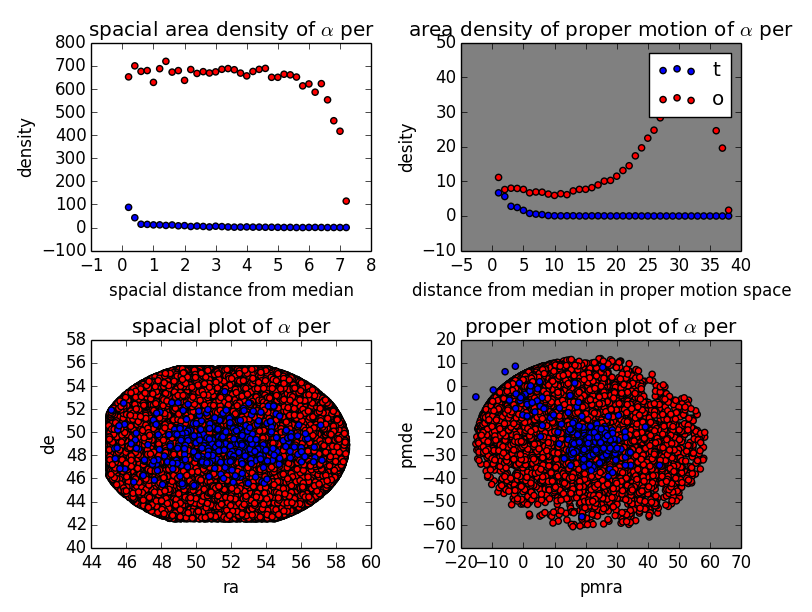
\includegraphics[width=0.9\textwidth]{quadplot}
\begin{multicols}{2}
\section{Introduction}
The $\alpha$ Persei Cluster is a relatively young open star cluster.  The age of $\alpha$ Per has not been adequately measured, and estimates range from $~30\mathrm{mY}$ to $~100\mathrm{mY}$.  Knowing the age of this cluster is relevant because better knowledge of the age of this cluster could aid in other astronomical estimates, and more knowledge of the cosmos is never a bad thing.  To begin I compiled a list known members from the previous surveys of the cluster, namely Deacon \& Hambly, and Prosser.  Additionally I added as known members stars from a survey conducted by [INSERT SURVEY NAME CUZ YOU FORGOT IT] in which the stars were: near the cluster center, at approximately the correct distance (estimated by comparison to an estimated isochrone), and x-ray detected, which is common of stars in the estimated age range of the cluster.  I then gathered data from the Urat1 survey of a square section of sky approximately centered on the center of the cluster.  

\section{Comparison of Candidate members}
I studied the distribution of stars in the set of known members to determine their distribution in 2-dimensional right ascension and declination space.  I modeled their distribution as a function of distance from the center of the distribution.  I calculated their area density in circular bins of expanding radii.

\begin{equation}
    D=\sqrt{\Delta\left( \alpha\cdot\mathrm{cos}(\delta)\right)^2+\Delta\delta^2}
\end{equation}

Were $\alpha$ is right ascension, and $\delta$ is declination.  I then calculated the number of known members in radius bins.  
\begin{equation}
    N_i=|\{D_i:r_i<=D<r_{i+1}|
\end{equation}

Finally I calculated the area density distribution as the number of stars in a bin divided by the area of the bin.
\begin{equation}
    P_i=\frac{N_i}{\pi(r_{i+1}^2-r_i^2)}
\end{equation}

Since cluster stars are gravitationally bound they should ideally move in a similar manner relative to Earth.  For this reason I re-purposed the methods above to calculate the area density in proper motion space. the only difference was that I approximated proper motion space to a flat two dimensional plane.  Thus the distance in proper motion space can be modeled as:
\begin{equation}
    \Delta\mathrm{PM}=\sqrt{\Delta\alpha_{\mathrm{PM}}^2+\Delta\delta_{PM}^2}
\end{equation}

Lastly I measured the distance of each member from a model isochrone created by Dotter, who used the pleiades cluster.  I still have an as of yet unresolved error in which the Isochrone I created only spans a small section of my candidate field, and relatively sharp upturns and downturns at the ends cause an extrapolation to rapidly approach infinite magnitude, and negative infinite magnitude, respectively.
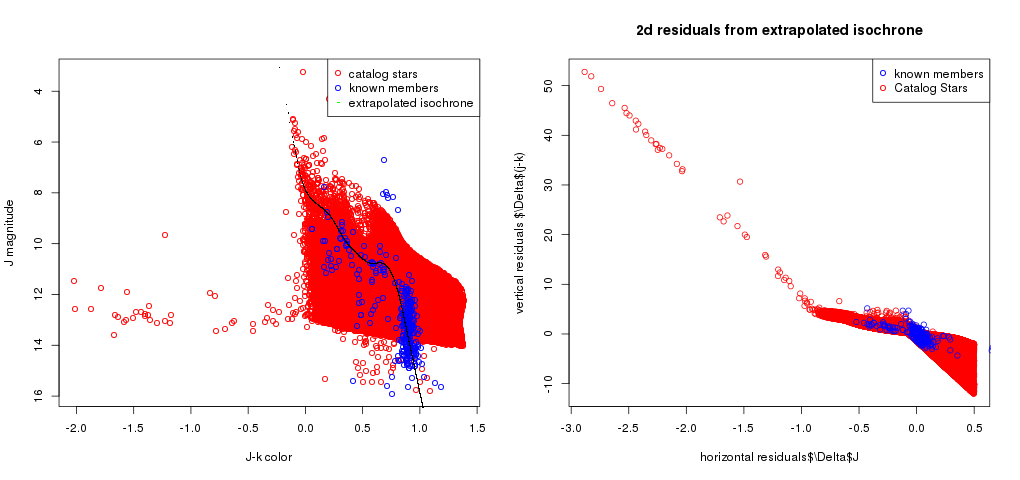
\includegraphics[width=.5\textwidth]{isochroneB}
\section{Work left undone}

Having found the median point in both spacial and proper motion space, we found the same radial distance, and area density for the candidate members.  I have yet to find a way to exactly translate the area density into probability.  I've begun theorizing a different heuristic to compute the isochrone, but that is little more than an idea.  I would likely create a basic polynomial in some small n dimensions, like 3 or 5 dimensions.  Then instead of minimizing the least squares distance from a point to the line in the classic sense, It would compute the shortest distance to some arbitrary point on the isochrone, not neccessarily the point corresponding to the respective x-value. Other than that I need to find a way of relating the radial area densities direcly to probabilities.   

\section{statistical identities}
The identities I intend to use to calculate membership probabilities are basic conditional probabilities:
\begin{equation}
P(A|B)=\frac{P(A\cap B)}{P(B)}
\end{equation}

This can be rearranged to solve for the probability of membership given radius, keeping in mind that calculating the probability of having a certain radius from the set of known members is a trivial undertaking.:
\begin{equation}
P(M|R)=\frac{P(R|M)P(M)}{P(R)}
\end{equation}

\section{roadmap}
Plot linear function with Gaussian of all objects to get an estimate of the number of cluster members.
\end{multicols}
\end{document}
